\documentclass{article}

% if you need to pass options to natbib, use, e.g.:
%     \PassOptionsToPackage{numbers, compress}{natbib}
% before loading neurips_2019

% ready for submission
% \usepackage{neurips_2019}

% to compile a preprint version, e.g., for submission to arXiv, add add the
% [preprint] option:
%     \usepackage[preprint]{neurips_2019}

% to compile a camera-ready version, add the [final] option, e.g.:
\usepackage[final]{neurips_2019}

% to avoid loading the natbib package, add option nonatbib:
%     \usepackage[nonatbib]{neurips_2019}

\usepackage[utf8]{inputenc} % allow utf-8 input
\usepackage[T1]{fontenc}    % use 8-bit T1 fonts
\usepackage{hyperref}       % hyperlinks
\usepackage{url}            % simple URL typesetting
\usepackage{booktabs}       % professional-quality tables
\usepackage{amsfonts}       % blackboard math symbols
\usepackage{nicefrac}       % compact symbols for 1/2, etc.
\usepackage{microtype}      % microtypography

\usepackage{latexsym, amssymb, amscd, amsthm, amsxtra, amsmath,amsthm }
\usepackage{graphics, graphicx, color}
\graphicspath{ {./images/} }
\usepackage[format=hang,indention=-1cm,small]{caption}
\usepackage[caption=false]{subfig}

\usepackage{natbib}

% MATH -----------------------------------------------------------
\newcommand{\norm}[1]{\left\Vert#1\right\Vert}
\newcommand{\abs}[1]{\left\vert#1\right\vert}
\newcommand{\set}[1]{\left\{#1\right\}}
\newcommand{\floor}[1]{\left\lfloor #1 \right\rfloor}
\newcommand{\Real}{\mathbb R}
\newcommand{\Nat}{\mathbb N}
\newcommand{\Int}{\mathbb Z}
\newcommand{\Complex}{\mathbb C}
\newcommand{\eps}{\varepsilon}
\newcommand{\To}{\longrightarrow}

\def\av{\mathbf a}
\def\bv{\mathbf b}
\def\cv{\mathbf c}
\def\dv{\mathbf d}
\def\ev{\mathbf e}
\def\fv{\mathbf f}
\def\gv{\mathbf g}
\def\hv{\mathbf h}
\def\iv{\mathbf i}
\def\jv{\mathbf j}
\def\gv{\mathbf g}
\def\kv{\mathbf k}
\def\lv{\mathbf l}
\def\mv{\mathbf m}
\def\nv{\mathbf n}
\def\ov{\mathbf o}
\def\pv{\mathbf p}
\def\qv{\mathbf q}
\def\rv{\mathbf r}
\def\sv{\mathbf s}
\def\tv{\mathbf t}
\def\uv{\mathbf u}
\def\vv{\mathbf v}
\def\wv{\mathbf w}
\def\xv{\mathbf x}
\def\yv{\mathbf y}
\def\zv{\mathbf z}

\def\Av{\mathbf A}
\def\Bv{\mathbf B}
\def\Cv{\mathbf C}
\def\Dv{\mathbf D}
\def\Ev{\mathbf E}
\def\Fv{\mathbf F}
\def\Gv{\mathbf G}
\def\Hv{\mathbf H}
\def\Iv{\mathbf I}
\def\Jv{\mathbf J}
\def\Kv{\mathbf K}
\def\Lv{\mathbf L}
\def\Mv{\mathbf M}
\def\Nv{\mathbf N}
\def\Ov{\mathbf O}
\def\Pv{\mathbf P}
\def\Qv{\mathbf Q}
\def\Rv{\mathbf R}
\def\Sv{\mathbf S}
\def\Tv{\mathbf T}
\def\Uv{\mathbf U}
\def\Vv{\mathbf V}
\def\Wv{\mathbf W}
\def\Xv{\mathbf X}
\def\Yv{\mathbf Y}
\def\Zv{\mathbf Z}

\newcommand{\alphav}{\mbox{\boldmath{$\alpha$}}}
\newcommand{\betav}{\mbox{\boldmath{$\beta$}}}
\newcommand{\gammav}{\mbox{\boldmath{$\gamma$}}}
\newcommand{\deltav}{\mbox{\boldmath{$\delta$}}}
\newcommand{\epsilonv}{\mbox{\boldmath{$\epsilon$}}}
\newcommand{\zetav}{\mbox{\boldmath$\zeta$}}
\newcommand{\etav}{\mbox{\boldmath{$\eta$}}}
\newcommand{\iotav}{\mbox{\boldmath{$\iota$}}}
\newcommand{\kappav}{\mbox{\boldmath{$\kappa$}}}
\newcommand{\lambdav}{\mbox{\boldmath{$\lambda$}}}
\newcommand{\muv}{\mbox{\boldmath{$\mu$}}}
\newcommand{\nuv}{\mbox{\boldmath{$\nu$}}}
\newcommand{\xiv}{\mbox{\boldmath{$\xi$}}}
\newcommand{\omicronv}{\mbox{\boldmath{$\omicron$}}}
\newcommand{\piv}{\mbox{\boldmath{$\pi$}}}
\newcommand{\rhov}{\mbox{\boldmath{$\rho$}}}
\newcommand{\sigmav}{\mbox{\boldmath{$\sigma$}}}
\newcommand{\tauv}{\mbox{\boldmath{$\tau$}}}
\newcommand{\upsilonv}{\mbox{\boldmath{$\upsilon$}}}
\newcommand{\phiv}{\mbox{\boldmath{$\phi$}}}
\newcommand{\varphiv}{\mbox{\boldmath{$\varphi$}}}
\newcommand{\chiv}{\mbox{\boldmath{$\chi$}}}
\newcommand{\psiv}{\mbox{\boldmath{$\psi$}}}
\newcommand{\omegav}{\mbox{\boldmath{$\omega$}}}
\newcommand{\Sigmav}{\mbox{\boldmath{$\Sigma$}}}
\newcommand{\Lambdav}{\mbox{\boldmath{$\Lambda$}}}
\newcommand{\Deltav}{\mbox{\boldmath{$\Delta$}}}

\newcommand{\Ac}{\mathcal{A}}
\newcommand{\Bc}{\mathcal{B}}
\newcommand{\Cc}{\mathcal{C}}
\newcommand{\Dc}{\mathcal{D}}
\newcommand{\Ec}{\mathcal{E}}
\newcommand{\Fc}{\mathcal{F}}
\newcommand{\Gc}{\mathcal{G}}
\newcommand{\Hc}{\mathcal{H}}
\newcommand{\Ic}{\mathcal{I}}
\newcommand{\Jc}{\mathcal{J}}
\newcommand{\Kc}{\mathcal{K}}
\newcommand{\Lc}{\mathcal{L}}
\newcommand{\Mc}{\mathcal{M}}
\newcommand{\Nc}{\mathcal{N}}
\newcommand{\Oc}{\mathcal{O}}
\newcommand{\Pc}{\mathcal{P}}
\newcommand{\Qc}{\mathcal{Q}}
\newcommand{\Rc}{\mathcal{R}}
\newcommand{\Sc}{\mathcal{S}}
\newcommand{\Tc}{\mathcal{T}}
\newcommand{\Uc}{\mathcal{U}}
\newcommand{\Vc}{\mathcal{V}}
\newcommand{\Wc}{\mathcal{W}}
\newcommand{\Xc}{\mathcal{X}}
\newcommand{\Yc}{\mathcal{Y}}
\newcommand{\Zc}{\mathcal{Z}}

\title{2022 IDL Midterm Report : \\ Microsoft Teams to Cloud Speech Enhancement}

% The \author macro works with any number of authors. There are two commands
% used to separate the names and addresses of multiple authors: \And and \AND.
%
% Using \And between authors leaves it to LaTeX to determine where to break the
% lines. Using \AND forces a line break at that point. So, if LaTeX puts 3 of 4
% authors names on the first line, and the last on the second line, try using
% \AND instead of \And before the third author name.

\author{%
%   David S.~Hippocampus\thanks{Use footnote for providing further information
%     about author (webpage, alternative address)---\emph{not} for acknowledging
%     funding agencies.} \\
  Hyun-Kuk Lim$^*$, Chanwoo Kim$^*$, Taeyoung Chang$^*$, Urvish Takker\thanks{Equal Contribution (random order)} \\ \\
%   Language Technology Institute\\
  Carnegie Mellon University\\
  Pittsburgh, PA 15213 \\
  \texttt{\{hyunkukl, chanwoo2, tchang3, udt\}@andrew.cmu.edu} \\
  % examples of more authors
  % \And
  % Coauthor \\
  % Affiliation \\
  % Address \\
  % \texttt{email} \\
  % \AND
  % Coauthor \\
  % Affiliation \\
  % Address \\
  % \texttt{email} \\
  % \And
  % Coauthor \\
  % Affiliation \\
  % Address \\
  % \texttt{email} \\
  % \And
  % Coauthor \\
  % Affiliation \\
  % Address \\
  % \texttt{email} \\
}

\begin{document}

\maketitle

\begin{abstract}
    With an increasing trend in remote work, conferencing platforms are significantly becoming important. 'Microsoft Teams', a popular platform for real-time conference, is one of them. 'Microsoft Teams' uses its speech enhancement model because noises can provide unsatisfactory quality of speech and eventually disrupt conversations. Suppressing them is crucial for a stable meeting. However, it is not easy due to some challenges. Since it has to be real-time, enhancement should proceed fast enough in time-limited context. And even if it suppresses noises well in technical manner, perceptual quality and intelligibility, which are essential since the enhanced output is specifically for human hearing, are not guaranteed. Hence, we improve (not yet done...) real-time speech enhancement model FullSubNet and Demucs. To ensure perceptual quality and intelligibility, auxiliary loss, which is defined using acoustic metrics, is also used. (Details about changes we make and the evaluations, and our beating MS teams in certain way)
\end{abstract}

\section{Introduction}

Speech enhancement has become one of the most important technologies in a remote working environment.  Meetings done through video conferencing platforms such as Zoom or Microsoft Teams are more prevalent than ever, and extracting clean speech from a noisy environment in real time is becoming more important to avoid interruptions during a conference. However, solely extracting clean speech in real-time is a difficult task, especially with imperfect information on the level of noise in the future. Furthermore, suppressing noise can also lead to the suppression of clean speech as well, removing essential parts of a conversation. Losing essential signals from speech may further degrade its quality, and to prevent this, noise must be filtered out the moment it is detected in audio. Thus, we want to build a model which would perform better in real time. 

Our goal is that when we get noisy speech data derived from synthesizing clean speech and noise, we want to build a model (where the basic structure is FullSubnet and some properties of Demucs are added in a clever way? Not determined yet…) that yields a speech close to the clean speech. In other words, we want to build a model that fulfills a noise suppression while perceptual quality and intelligibility of the output is at least competitive with the noise suppression output of Microsoft Teams. 

Here, the input is a spectrogram transformed from the synthesized speech file. The spectrogram can be viewed as a 2D tensor of a shape with (T, F). For each time $t \in \{1, \cdots, T\}$, the wave form of short time segment near $t$ is Fourier-transformed (STFT) and the absolute value of this short term fourier transform at each frequency $f$ is stored as F-dimensional vector. Our model is defined as mapping a spectrogram of noisy speech data to the training target cIRM which stands for complex Ideal Ratio Mask(\cite{CIRM}). Since the desired output of cIRM can be viewed as the complex ratio of clean speech spectrum to noisy speech spectrum, training via the loss of measuring distance of actual output and the desired output can be interpreted as knowing well where the noise exists in time-frequency domain so that we can suppress such noise.


\section{Related Works}
\label{related_works}

\subsection{Demucs}

The authors of this paper(\cite{Demucs}) utilize convolutional and recurrent neural networks to separate noise from the clean speech in waveform audio. By processing corrupted audio through convolutional encoder-decoder architecture with skip-connections they propose that clean speech can be extracted from latent representations of input audio. Furthermore, to account for sequential information in the audio a recurrent neural network is injected between encoders and decoders, which the decoder uses to reconstruct clean speech. To account for real-time noise suppression the authors accumulate standard deviations of audios only up to the current position for normalization, with paddings to account for a 3ms lookahead.


\subsection{FullSubNet}

This paper(\cite{fullsubnet}) introduces a full-band and sub-band fusion model, FullSubNet, which enhances single-channel speech. Full-band model has its strength in finding global spectral patterns and cross-band dependencies. On the other hand, sub-band model has its strength in finding local spectral patterns and stationarity, which is an important factor that distinguishes noises from clean speech. Since both models have their own advantages, FullSubNet stacks both models to take both advantages. The whole speech spectrogram goes through a full-band model, and the output is concatenated with sub-band unit. Then the concatenated ones become frequency-wise inputs of the sub-band model. Hence, the sub-band model can find local patterns with complementary information captured from the full-band model. Besides, this model exceeds the high-ranked models in the DNS Challenge (INTERSPEECH 2020).

\subsection{eGeMAPS}

This paper(\cite{GeMAPS}) suggests a minimalistic set of standard acoustic parameters such as Pitch, Jitter, Shimer, Loudness, Harmonics-to-Noise Ratio, and Harmonic difference. It is selected based on three criteria: the potential to discern physiological changes in voice production, the success in the past literature, and the theoretical importance. Through the experiments, the paper argues that, unlike the large brute-forced feature sets, the minimalistic parameter sets might reduce the danger of damaging generalization capabilities to unseen data. The authors proposed these parameters as the common baseline for evaluating future research. 

\subsection{Auxiliary Loss using eGeMAPS}

Although noise suppression or removal is a significant part of the speech enhancement, we should also pay attention to retaining the perceptual quality and intelligibility of the speech signal. Traditionally, deep neural networks based approaches are trained exploiting pointwise differences in time-domain or time-frequency-domain, but this loss has been shown to be insufficient to bring out high perceptual quality of enhanced speech. To improve perceptual quality, two papers(\cite{eGeMapsLoss}, \cite{TAPloss}) suggest adding the loss derived by the difference between clean speech and enhanced speech with respect to eGeMAPS features as an auxiliary objective. For expressing the eGeMAPS features, the first one(\cite{eGeMapsLoss}) uses summary statistics of acoustic parameters, known as the functionals, per utterance, whereas the second one(\cite{TAPloss}) utilizes temporal acoustic parameters, or the low-level descriptors (LLD), of each utterance, allowing the optimization at each time step. Also, both papers propose to train eGeMAPS prediction network that can be plugged into other learning pipelines, since existing calculations for eGeMAPS are non-differentiable.

\section{Model Description}

\subsection{FullSubNet}

The model is a combination of a full-band model $G_{full}$, and a sub-band model $G_{sub}$. An input for $G_{full}$ is a sequence of noisy full-band magnitude spectral features
\begin{equation}
    \widetilde{\textbf{X}} =         (\textbf{X}(1),\cdots,\textbf{X}(t),\cdots,\textbf{X}(T))\in \mathbb{R}^{F\times{T}}.
\end{equation}
And each feature consists of complex-valued time-frequency (T-F) bins of a certain time frame $t$
\begin{equation}
    \textbf{X}(t) = \left [ \left| X(t,0)\right|,\cdots,\left| X(t,f)\right|,\cdots, \left|X(t,F-1)\right| \right ]^{T}\in \mathbb{R}^{F}.
\end{equation}
The full-band model $G_{full}$ outputs a spectral embedding with the size same as $\widetilde{\textbf{X}}$, which captures the global context. Then the part of the embedding corresponding to each frequency is concatenated with the noisy sub-band signal of that frequency. Note that a noisy sub-band signal of a frequency is composed of the frequency and $2\times{N}$ adjacent frequencies. Hence, there are total $F$ sequences as the inputs for $G_{sub}$. An input sequence for the frequency $f$ is
\begin{equation}
    \widetilde{\textbf{x}}(\mathit{f}) =         (\textbf{x}(1,\mathit{f}),\cdots,\textbf{x}(t,\mathit{f}),\cdots,\textbf{x}(T,\mathit{f}))\in \mathbb{R}^{(2N+2)\times{T}}
\end{equation}
where
\begin{equation}
\textbf{x}(t,f) = \left [ \left| X(t,f-N)\right|,\cdots,\left| X(t,f)\right|,\cdots, \left|X(t,f+N)\right|, G_{full}(\left|(X(t,f)\right|)\right ]^{T}\in \mathbb{R}^{2N+2}.
\end{equation} 
Finally for each frequency, the sub-band model $G_{sub}$ takes each input sequence and predicts a complex Ideal Ratio Mask (cIRM) sequence which distinguishes clean speech with respect to each frequency.

The full-band and sub-band models have basically the same structure with two unidirectional LSTM layers and one fully connected layer. The difference is that full-band model has 512 hidden units in each LSTM layers and uses ReLU activation after the fully connected layer, whereas sub-band model has 384 hidden units in each LSTM layers and uses no activation. Even though there are F different frequencies, there is only one unique sub-band model $G_{sub}$. 


\subsection{DEMUCS}
DEMUCS utilizes convolutional encoder-decoder architecture with U-net skip connections \cite{UNet} with a recurrent neural network in between the last encoder layer and the first decoder layer to capture sequential information of audio. Given noisy audio $\xv \in \mathbb{R}^T$ where x is corrupted from $\yv \in \mathbb{R}^T$ using an additive noise $\nv \in \mathbb{R}^T$, or $\xv = \yv + \nv$, the goal of the model is to find $f$ such that $f(\xv) \approx \yv$. 

Both the encoder and the decoder architectures consist of two convolution layers. The encoder's first convolution extracts representation of the input or the output of the previous layer and the second doubles the number of channels using a 1x1 convolution, or channel-wise pooling, and the output is used as input into the next encoder/LSTM layer and the corresponding decoder layer following U-net architecture. ReLU activation and GLU activation are used respectively. The decoder's architecture is an inverse operation of the encoder, where the first is the 1x1 convolution followed by GLU and the second is a transposed convolution. The decoder takes as input output from the previous decoder or LSTM layer and the output from the connected encoder to create a waveform of enhanced audio, or $f(\xv)$. The LSTM network $R$ captures sequential information, or a non-linear transformation, of the latent representation $\zv$ from the last encoder layer, denoted $\hat \zv = R(\zv) = LSTM(\zv) + \zv$, which goes into the first decoder layer.


\section{Dataset}

We will use the dataset from the github repository of \href{https://github.com/microsoft/DNS-Challenge}{DNS Challenge 2020}. There is an explanation for the dataset in \cite{DNSchallenge2020}. 

For training data, we will get the noisy speech dataset by synthesizing clean speech and noise. The clean speech dataset comes from the public audiobooks dataset called Librivox. It has recordings over 10,000 public domain audiobooks by 11,350 speakers where majority of them are in English. Many of these recordings have excellent speech quality, but still some are of poor speech quality with speech distortion, background noise and reverberation. Thus, DNS Challenge 2020 has filtered the clean speech data based on the speech quality, which is measured by the Mean Opinnion Score (MOS), and chose only the upper quartile with respect to MOS as the clean speech dataset. The resulting dataset has 500 hours of speech from 2150 speakers and all the filtered clips are split into segments of 10 seconds.

The noise clips were selected from Audioset and Freesound. Audioset is a collection of about 2 million human-labeld 10 second sound clips. They are drawn from YouTube videos and belong to about 600 audio events. Since certain audio event classes such as music and speech are overrepresented in the Audioset, DNS Challenge 2020 has tried to balance the dataset by sampling so that each class audio event class has at least 500 clips. Also, DNS Challenge 2020 has removed the clips with any kind of speech activity since speech-like noise can bring out the suppression of speech while the trained model tries to suppress speech-like noise. The resulting noise dataset has about 150 audio classes and 60,000 clips. An additional 10,000 noise clips from Freesound are also augmented to the dataset.

The noisy speech dataset is created by adding clean speech and noise at various SNR levels. (Synthesizing the clean speech and noise : same method as the paper? Or new method?)

Although what we observe in the real world is not perfectly expressed by the synthetic dataset, we take advantage of the synthetic dataset since most of the speech enhancement (SE) models require a clean reference for utilizing objective metrics such as PESQ or STOI.

For the test set, we can use synthetic test dataset which adds the clean speech from the Graz University's clean speech dataset and noise clips from the Audioset and Freesound, which are not present in the training set. Since these synthetic clips come with ground truth references which are the clean speech data, we can evaluate the method using objective metrics such as PESQ and STOI. Whereas for the test set, or `blind' test set, there is no ground truch references provided. We can use this set for the final evaluation using subjective metrics.

Here, for our problem, we can write $x = y+n$ where $y$ is the clean speech, $n$ is the noise, and the $x$ is the synthesized noisy speech. Simply put, $x$ is the input for our model and the $y$ is the desired output of our model. If we denote $\hat y$ as the actual output of our model and $y^\star$ as the output from the Microsoft Teams platform, then we want for the divergence of $\hat y$ and $y$  to be smaller than that of $y^ \star$ and $y$. In this way, we can measure how well our noise suppression model works compared to Microsoft Teams.

\section{Evaluation Metric}

\begin{tabular}{ |p{2.5cm}||p{11cm}|}
    \hline
    \multicolumn{2}{|c|}{Evaluation Metric List} \\
    \hline
    Metric &  Mathematical Expression\\
    \hline
    \vspace{2cm}\textbf{STOI}  & $$STOI = \frac{1}{JM}\sum_{j, m} d_{j,m}$$  \begin{itemize}
        \item $J$ : the number of one-third octave bands (frequency)
        \item $M$ : the total number of frames (time)
        \item $d_{j,m}$ : sample correlation between $\xv_{j,m}$ and $\overline{\yv}_{j,m}$
        \item $\xv_{j,m}$ : the short-time temporal envelope of the clean speech
        \item $\overline{\yv}_{j,m}$ : the short-time temporal envelop of the (normalized and clipped) degraded speech 
    \end{itemize} \\ 
    \hline
    \vspace{1.2cm}\textbf{PESQ} &   $$PESQ = a_0 + a_1 D_{ind} + a_2 A_{ind}$$
    \begin{itemize}
        \item $D_{ind}$ : average disturbance
        \item $A_{ind}$ : asymmetric average disturbance 
        \item $a_0, a_1, a_2$ : $a_0$ is set as 4.5 and $a_1, a_2 <0$ can be modified for the given task
    \end{itemize}  \\
    \hline 
    \vspace{2cm} \textbf{fwSegSNR} & $$fwSegSNR = \frac{10}{M} \sum_{m=1}^{M-1}\frac{\sum_{j=1}^K W(j,m)\log_{10} \frac{\abs{X(j,m)}^2}{(\abs{X(j,m)} - \abs{\hat X(j,m)})^2} }{\sum_{j=1}^K W(j,m)} $$
    \begin{itemize}
        \item $K$ : the number of bands 
        \item $M$ : total number of frames 
        \item $\abs{X}$ : weighted (by a Gaussian shaped window) clean signal spectrum 
        \item $W$ : weight on $j$-th frequency and $m$-th frame, which is exponential of $\abs{X}$
    \end{itemize}\\
    \hline
\end{tabular}

\vspace{1cm}

STOI(\cite{STOI}) stands for a short-time objective intelligence measure. Essentially it measures the average of every correlation coefficient between each of short-time segments of DFT(discrete Fourier transform)-based band for clean speech and the output of noise reduction from the noisy speech input. 

Perceptual Evaluation of Speech Quality (PESQ)(\cite{PESQ}) is a metric used for obtaining Mean Opinion Scores (MOS) of speech in an audio. This objective metric, ranging from -0.5 to 4.5, measures the quality of an audio based on a sum of disturbances in the audio, and while it is not intended for speech enhanced by noise suppression, we follow \cite{microsoftTeams}, our baseline model, to compare our model’s performance.

% SDR or Speech to Distortion Ratio: Distortion is unwanted signal correlated with the input signal. It's absent until the signal appears, and is usually not significant until the signal is occupying most of the dynamic range of the system. This can be a very good metric to track as distortion is something we can reduce and it might lead to clean speech results.

fwSegSNR(\cite{evalMetrics}), Frequency weighted Segmental Signal-to-Noise Ratio, is a generalized short time performance measure. It gives each frequency’s SNR two kinds of weights. First, static frequency weighting that is derived from known psycho-acoustic properties of hearing. Second, dynamic frequency weighting which is related to the speech production mechanism.

\section{Loss Function}

For this section, we shall use the notations below.
\begin{itemize}
    \item Time domain
    \begin{itemize}
        \item $\yv\in \Real^T$ : a clean speech waveform
        \item $\nv\in \Real^T$ : a noise waveform
        \item $\xv = \yv + \nv$ : a noisy speech waveform
    \end{itemize}
    \item Time-Frequency domain
    \begin{itemize}
        \item $\Yv \in \Complex^{T\times F}$ : a complex spectrogram for clean speech
        \item $\Nv \in \Complex^{T\times F}$ : a complex spectrogram for noise 
        \item $\Xv = \Yv + \Nv$ : a complex spectrogram for noisy speech 
    \end{itemize}
    \item Speech-Enhancement model
    \begin{itemize}
        \item A speech enhancement model $G$ maps $\xv\in \Real^T$ to $\hat \yv\in \Real^T$ where $\hat \yv$ is a waveform of enhanced speech. 
    \end{itemize}
\end{itemize}

\subsection{Loss function for Demucs}
Given $\yv$ and $\hat \yv$, the loss $\Lc_{Demucs}$ can be expressed as 
\[\Lc_{Demucs} = \Lc_{Wave} + \lambda \Lc_{Spectrogram}\] Here, $\Lc_{Wave}$ is a waveform loss \[\Lc_{Wave}(\yv, \hat \yv) = \norm{\yv - \hat \yv}_1\] and $\Lc_{Spectrogram}$ is a multi-resolution STFT loss
\begin{equation*}
    \Lc_{Spectrogram}(\yv, \hat \yv) = \Lc_{sc}(\yv, \hat \yv) + \Lc_{mag}(\yv, \hat \yv) 
\end{equation*} 
where the spectral convergence loss and magnitude loss are given as
\begin{equation*}
    \Lc_{sc}(\yv, \hat \yv) = \frac{\norm{\abs{\Yv} - |\hat \Yv|}_F}{\norm{\abs{\Yv}}_F} \quad \text{and} \quad \Lc_{mag}(\yv, \hat \yv) = \frac 1T \norm{\log\abs{\Yv} - \log |\hat \Yv|}_1
\end{equation*}

\subsection{Loss function for FullSubNet}

Given noisy waveform $\xv$ and clean waveform $\yv$, we can get complex spectrogram $\Xv$ and $\Yv$ respectively. FullSubNet takes noisy spectrogram $\Xv$ as an input and the output is the estimated complex Ideal Ratio Mask(cIRM) $\hat \Mv\in \Complex^{T \times F}$ while the target output is complex Ideal Ratio Mask $\Mv \in \Complex^{T \times F}$ such that $\Yv = \Mv \odot \Xv$ where $\odot$ is an element-wise multiplication. FullSubNet uses the mean squared error between $\Mv$ and $\hat \Mv$ as the loss $\Lc_{cIRM}$.

\subsection{Adding auxiliary loss}

For the objective function of both of enhancement models, Demucs and FullSubNet, an auxiliary loss regarding acoustic parameters can be added to improve their perceptual quality and intelligibility.

\[\Lc_{new} = \Lc_{original} + \gamma \Lc_{acoustic} \]

For $\Lc_{acoustic}$, \cite{eGeMapsLoss} suggests $\Lc_{eGeMAPS}$ while \cite{TAPloss} proposes $\Lc_{TAP}$. 

$\Lc_{eGeMAPS}$ is designed to narrow the difference between the eGeMAPS functionals outputs (which are $D=88$ dimensional vectors) of the clean speech and enhanced speech. Given clean waveform $\yv$ and enhanced waveform $\hat \yv$, the eGeMAPS loss is represented as the following.

\[\Lc_{eGeMAPS} = \norm{\ev - \hat \ev}_2^2 = \norm{g(\yv) - h_\phi(\hat \Yv)}_2^2 \]

Here, $g$ is original non-differentiable function to calculate eGeMAPS and $h_\phi$ is a neural network parameterized by weights $\phi$, which is an estimator for eGeMAPS functionals. 

On the other hand, $\Lc_{TAP}$ is designed to narrow the difference between the outputs of 25 temporal acoustic parameters with $T$ discrete time frames of the clean speech and enhanced speech. Given clean waveform $\yv$ and enhanced waveform $\yv$, the TAP loss is expressed as the following.

\[\Lc_{TAP} = \text{MAE}(A_\psi(\yv) \odot \sigma(\omegav) , A_\psi(\hat \yv) \odot \sigma(\hat \omegav) ) \]

Here, $A_\psi$ takes a signal input and outputs the temporal acoustic parameter estimates using a recurrent neural network parameterized by $\psi$. Also, $\omegav$ expresses the frame energy weights, which is derived from the Parseval's identity ; $\wv = \frac 1F \sum_{f} \abs{\Yv(f)}^2$ where $\Yv(f) \in \Complex^T$ for each $f=1, \cdots, F$ and $\Yv = (\Yv(1), \cdots, \Yv(F))$. Note that $\sigma$ denotes the sigmoid function.

We aim to fine-tune two pre-trained models (Demucs and FullSubNet) under the supervision of loss that we have just mentioned in order to get enhanced speech with high quality in terms of perception and intelligibility. During backward propagation of this fine-tuning process, the weight parameters $\phi$ and $\psi$ of estimator networks for eGeMAPS functionals and TAP are trained prior to the fine-tuning and stays frozen while the enhancement model weight parameters are optimized.

\section{Baseline}

Microsoft Teams is a business communication platform developed by Microsoft, of which usage share keeps increasing so that its number of users reaches 270million in 2022 (\href{(https://www.businessofapps.com/data/microsoft-teams-statistics/)}{Source}). It mainly provides lots of features that support live speech in meetings, calls, and so on. Hence, the need for speech enhancement is inevitable. So we aim to improve it more and adopt Microsoft Teams as the baseline of our model. Although papers from Microsoft including \cite{microsoftTeams} suggest Microsoft’s research into an extension of the Demucs architecture, the exact model used in Microsoft Teams is not publicly available due to the confidentiality of their research. However, we can still set our model’s baseline as the model used in Microsoft Teams by obtaining the suppressed audio by inputting the audio through their platform. To minimize the noise that could come from recording audio through a microphone, we inject the corrupted audio through a virtual microphone to simulate the inference stage of inputting audio files into Microsoft’s model.

\section{Analysis of Current Findings}

Analysis is critical to understanding the state-of-art of the present models and system. We employ the dataset from DNS Challenge 2020 \cite{DNSchallenge2020}, specifically the test set that consists of 150 clean and synthetically noisy audio pairs. The noisy data is as input to the FullSubNet and Demucs models for our analysis of enhancement. 

\begin{table}[!ht]
    \centering
    \caption{Statistics of Evaluation Metrics of Noisy and Enhanced Audio}
    \begin{tabular}{|l|l|l|l|l|l|l|l|l|l|}
    \hline
        Metric & Statistics & Noisy & DEMUCS & FullSubNet   \\ \hline
        PESQ & mean & 1.5822 & 2.6447 & 2.8885   \\ \hline
        PESQ & std & 0.4575 & 0.6332 & 0.6719  \\ \hline
        STOI & mean & 0.9152 & 0.9652 & 0.9641 \\ \hline
        STOI & std & 0.0646 & 0.0328 & 0.0349   \\ \hline
        fwSNRSeg & mean & 12.6233 & 17.1348 & 16.9617   \\ \hline
        fwSNRSeg & std & 4.9981 & 3.7549 & 4.3833  \\ \hline
    \end{tabular}
\end{table}

Table 1 shows the mean and standard deviation of PESQ, STOI and fwSNRSeg over 150 audio signals of each audio set. We calculate these metrics between the clean audio set and each of noisy set, enhanced set using DEMUCS, and enhanced set using FullSubNet. We find according to the statistics that both DEMUCS and FullSubNet improves the noisy audio as all three metrics increase for the outputs of DEMUCS and FullSubNet. PESQ value represents the perceptual evaluation of speech quality and optimal value for the same is 4.5 and the PESQ value nearer to 4.5 implies better audio quality. It is observed that the mean PESQ values of both Demucs and FullSubNet are significantly higher than the mean PESQ value of noisy data. 

Similarly, we observe that statistics for STOI and fwSNRSeg give similar results. STOI denotes correlation with the clean speech and higher STOI implies output is more correlated to the clean speech suggesting improvement over noisy set. In the results we observe that FullSubNet and Demucs have higher mean values for STOI over noisy. fwSegSNR denotes ratio of audio signal over noise, and higher fgSegSNR shows that the level of noise is lower. As anticipated, Demucs and FullSubNet have higher mean fwSegSNR values compared to the mean fwSegSNR value for the noisy data. 

\begin{figure}[h]
    \centering
    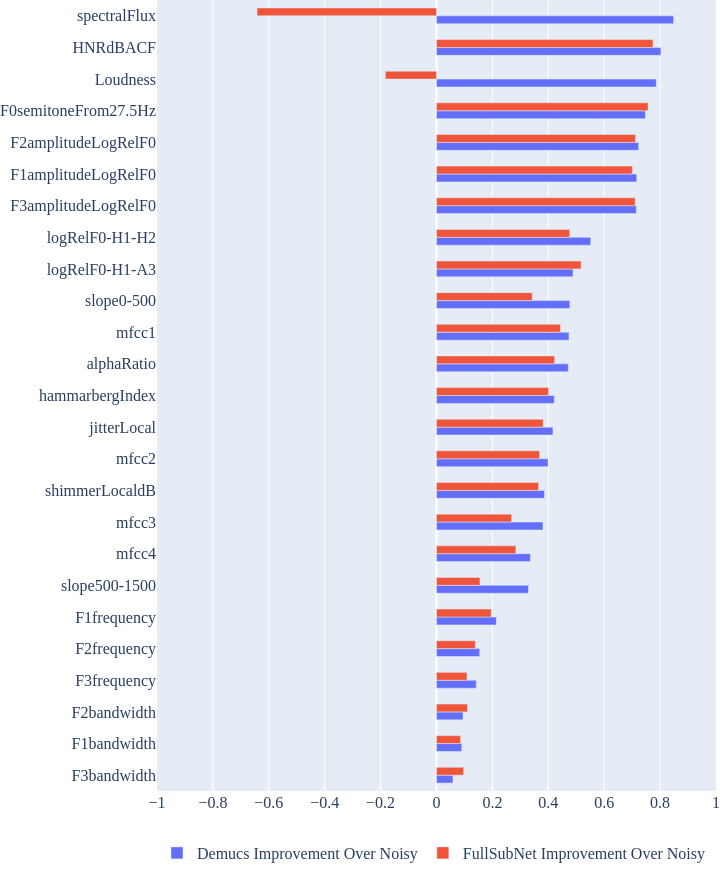
\includegraphics[width = 0.6 \textwidth]{egemaps_improvement_lowlevel.png}
    \caption{Graph of improvements by DEMUCS and FullSubNet over noisy audio on 25 temporal acoustic parameters. The improvement is a percentage difference between the MAE of parameters for the noisy set and the MAE of each model's enhanced audio set.}
\end{figure}

eGeMAPS suggest that traditional evaluation metrics might not be sufficient to gauge the overall perceptual quality of the speech. Thus, 25 temporal acoustic parameters, or low-level descriptors, are introduced to measure the overall perceptual quality of the speech. In the Figure 1 , we analyze all parameters over small windows of audio and calculate the Mean Absolute Error (MAE) of each eGeMAPS parameter between the models' output and the original clean speech. We perform the same calculation for noisy data as well and obtain the improvement of enhancement models as percentage difference between the MAE from noisy data and the MAE from each model output.

We expect this value to be positive as we anticipate MAE for noisy data to be higher than the MAE calculated by respective model output and from the figure we can see the results are mostly as expected. However, for features such as spectralFlux and Loudness, the error between output of FullSubNet and the clean speech was larger than the error between noisy and clean audio.

\begin{figure}[h]
    \centering
    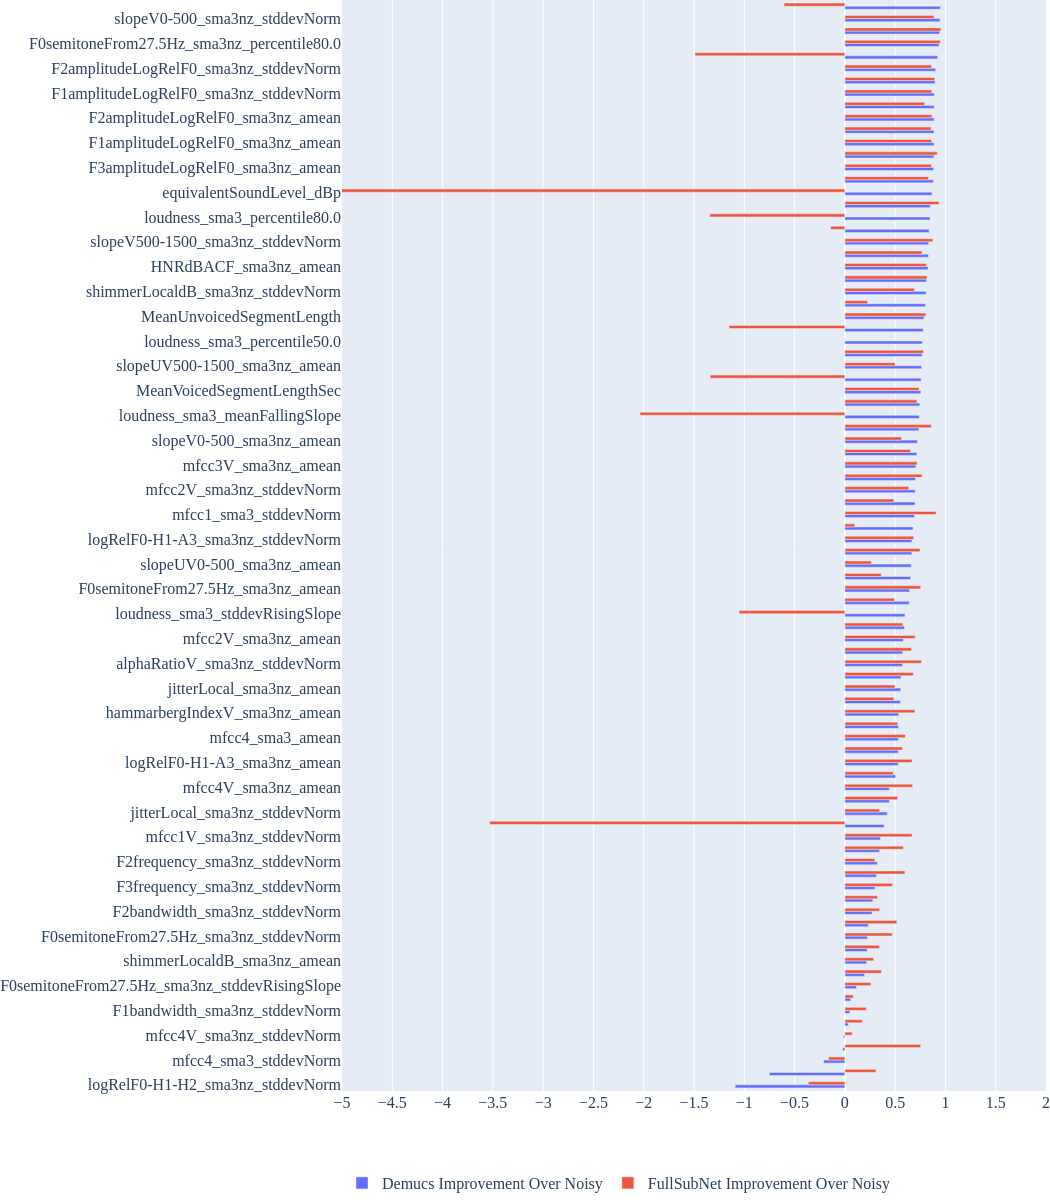
\includegraphics[width = 0.8 \textwidth]{egemaps_improvement_functionals.png}
    \caption{Graph of improvements by DEMUCS and FullSubNet over noisy audio on different statistics of temporal acoustic parameters. These statistics, referred to as the functionals, include mean, standard deviation, and percentiles of the eGeMAPS parameters. The improvement is derived using the same calculation as Figure 1.}
\end{figure}

Figure 2 shows improvement by DEMUCS and FullSubNet in different statistics of temporal acoustic parameters, or the functionals. Although Figure 1 shows the percentage acoustic improvements in low-level descriptors, improvements in the functionals would convey that the overall statistics of clean speech and enhanced speech are similar, implying better performance. Although Figure 2 shows that most statistics have improved from the noisy set, the enhanced set from both DEMUCS and FullSubNet were significantly different in some some of the functionals such as F1 bandwidth or loudness.

While the evaluation metrics from Table 1 show that both DEMUCS and FullSubNet significantly improves the quality of synthetically noisy audio, the percentage audio improvement plots for the low-level descriptors and the functionals suggest that the model outputs fall behind in some of the parameters. We can infer from these results that improving these parameters to be closer to the original clean speech would provide cleaner audio signal as well as better perceptual quality of the audio.

\bibliographystyle{plain}
\bibliography{references}


\end{document}